\chapter{Lezione 5}
\label{chap:lezione_05} 

\begin{flushright}
\textit{Data: 09/10/2025}
\end{flushright}

\section{Rottura di simmetria}

Una singola \textbf{configurazione} è definita assegnando un valore a ciascuno spin del sistema. Ad esempio, in un sistema con $10^{23}$ spin, una configurazione potrebbe essere: $\sigma_1 = +1, \sigma_2 = +1, \sigma_3 = -1, \dots$. 

Uno \textbf{stato} è l'insieme delle configurazioni che si troverebbero tipicamente all'equilibrio per un dato valore dei parametri esterni, come l'energia o la magnetizzazione.

\vspace{0.5cm}

\begin{tcolorbox}[colback=yellow!30,  
                  colframe=yellow!50!orange,  
                  boxrule=0.8pt, 
                  arc=3pt,  
                  top=4pt, bottom=4pt, left=6pt, right=6pt,
                  enhanced,
                  sharp corners=south]
Per temperature inferiori alla temperatura critica ($T < T_c$) e nel limite di volume infinito ($V \to \infty$), il sistema presenta una magnetizzazione spontanea non nulla ($m \neq 0$). In questa condizione, la simmetria è rotta. Se prepariamo il sistema e lo osserviamo, troveremo una magnetizzazione definita. Per ogni configurazione $C$ con magnetizzazione $m(C)$, esiste una configurazione $\tilde{C}$ (ottenuta invertendo tutti gli spin) tale che la sua magnetizzazione $m(\tilde{C})$ è uguale a $-m(C)$.
\end{tcolorbox} 

Quando prepariamo un sistema, ad esempio partendo da una temperatura infinita (una configurazione disordinata) e lo raffreddiamo, la probabilità di finire in uno stato con magnetizzazione positiva è $\frac{1}{2}$, e la stessa probabilità c'è di finire in uno stato con magnetizzazione negativa. Questo accade perché nella configurazione iniziale ad altissima temperatura, ci sarà casualmente una leggera maggioranza di spin positivi o negativi che, durante il processo di raffreddamento, guiderà il sistema verso uno stato finale con magnetizzazione positiva o negativa.

La simmetria è rotta perché, osservando il sistema in un dato istante e in un dato campione, troveremo che una specifica magnetizzazione è selezionata: il sistema si troverà nello stato con magnetizzazione "più" o in quello con magnetizzazione "meno".

\subsection{Stati puri e miscele statistiche}

Definiamo \textbf{stato puro} uno stato che osserviamo all'equilibrio. A temperature elevate, sopra la temperatura critica, il sistema non presenta una magnetizzazione netta. Se invece andiamo al di sotto della temperatura critica ($T < T_c$) e osserviamo il sistema in un dato momento, lo troveremo magnetizzato positivamente o negativamente. Gli stati puri sono quindi lo stato "+" e lo stato "-".

Lo stato con magnetizzazione totale nulla non è uno stato puro. Esso è in realtà una \textbf{miscela statistica} dei due stati puri.
\begin{equation}
| \psi \rangle_{T<T_c} = \frac{1}{2} (|+\rangle + |-\rangle)
\end{equation}
Questo stato con $m=0$ rappresenta una media su molte configurazioni del sistema, ma non è uno stato che si osserverà mai in un singolo esperimento nel limite di volume infinito. A $T < T_c$, gli stati puri sono $|+\rangle$ e $|-\rangle$.

Questa rottura di simmetria è valida rigorosamente solo nel \textbf{limite di volume infinito} ($V \to \infty$). Se il volume è finito, c'è sempre una probabilità, sebbene estremamente piccola e decrescente con il volume, che il sistema transisca da uno stato di magnetizzazione positiva a uno di magnetizzazione negativa. Il tempo necessario per una tale transizione diverge con il volume. Nel limite di volume infinito, una volta che il sistema si trova nello stato "+", non c'è modo di passare allo stato "-", poiché il costo energetico per attraversare configurazioni intermedie sarebbe infinito.

\subsection{Singolarità e ordine dei limiti}

La discrepanza tra un'Hamiltoniana simmetrica e stati non simmetrici può avvenire solo in presenza di una \textbf{singolarità}, che emerge nel limite di volume infinito.
\begin{equation}
\langle m \rangle = \frac{\sum_{\{\sigma\}} m(\{\sigma\}) e^{-\beta H}}{\sum_{\{\sigma\}} e^{-\beta H}}
\end{equation}
Questa espressione non è simmetrica, mentre $H$ lo è. Questa rottura di simmetria può avvenire solo se c'è una singolarità legata al fatto che il volume è infinito. Quando si sommano infiniti termini, anche se ognuno è regolare, la somma può sviluppare una singolarità.

A causa di queste singolarità, è fondamentale prestare attenzione all'ordine dei limiti.
\begin{itemize}
    \item Se prima poniamo $h=0$ e poi mandiamo il volume a infinito ($V \to \infty$), troveremo sempre una magnetizzazione media nulla, $m=0$.
    \item Al contrario, per osservare la magnetizzazione spontanea, dobbiamo prima mandare il volume a infinito ($V \to \infty$) per un $h$ fissato (anche se piccolo), e solo successivamente prendere il limite di $h \to 0$.
\end{itemize}
Quindi, l'operazione corretta è:
\begin{equation}
m_s = \lim_{h \to 0^+} \lim_{V \to \infty} m(h,V)
\end{equation}

\subsection{Proprietà della funzione di energia libera}

Consideriamo l'energia libera $f(h)$. Essa ha le seguenti proprietà:
\begin{enumerate}
    \item È una funzione pari di $h$: $f(h) = f(-h)$.
    \item La magnetizzazione è data dalla derivata dell'energia libera rispetto al campo magnetico:
    \begin{equation}
    m(h) = -\frac{\partial f(h)}{\partial h}
    \end{equation}
    Essendo la derivata di una funzione pari, $m(h)$ è una funzione dispari: 
    
    $m(h) = -m(-h)$.
\end{enumerate}

\begin{figure}[h!]
    \centering
    \begin{minipage}[b]{0.45\textwidth}
        \centering
        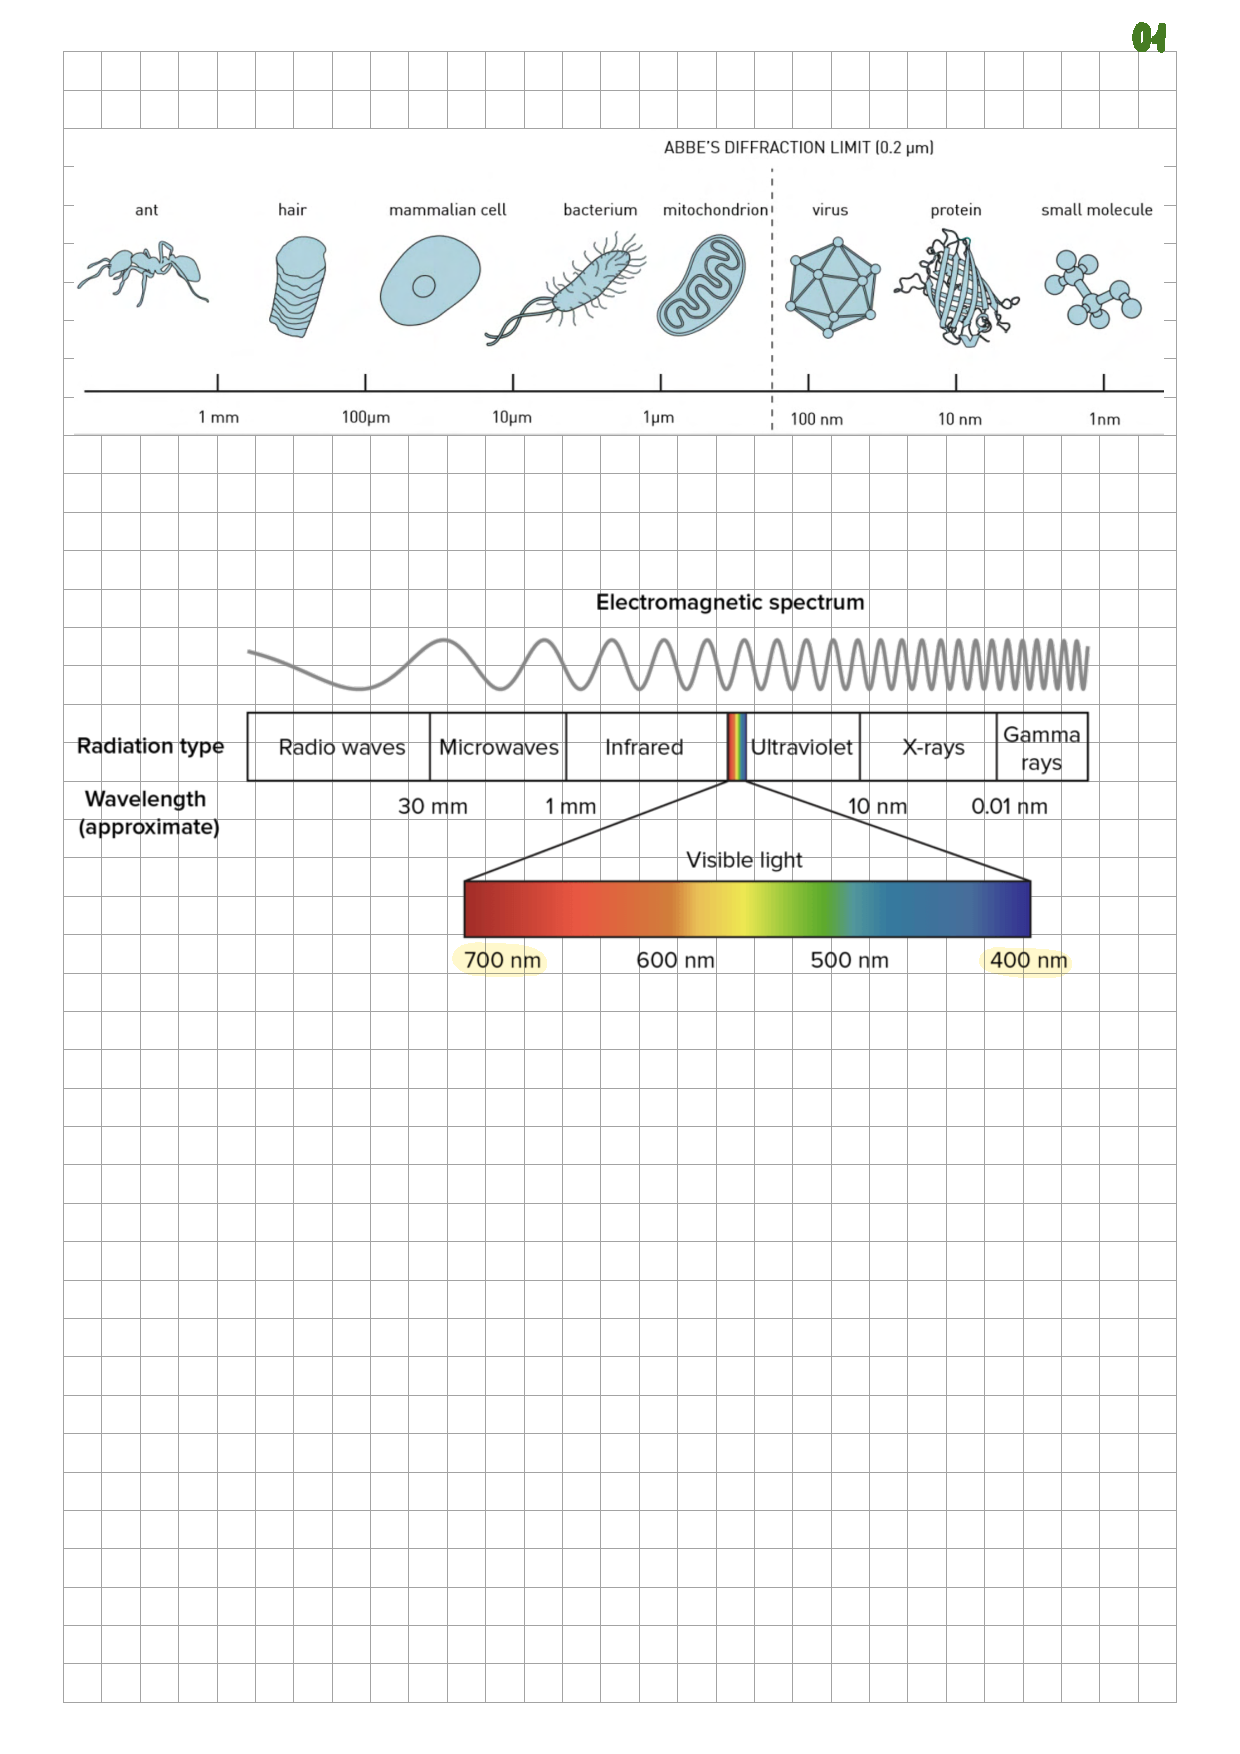
\includegraphics[width=\textwidth]{pics/01.png}
    \end{minipage}
    \hfill
    \begin{minipage}[b]{0.5\textwidth}
        \centering
        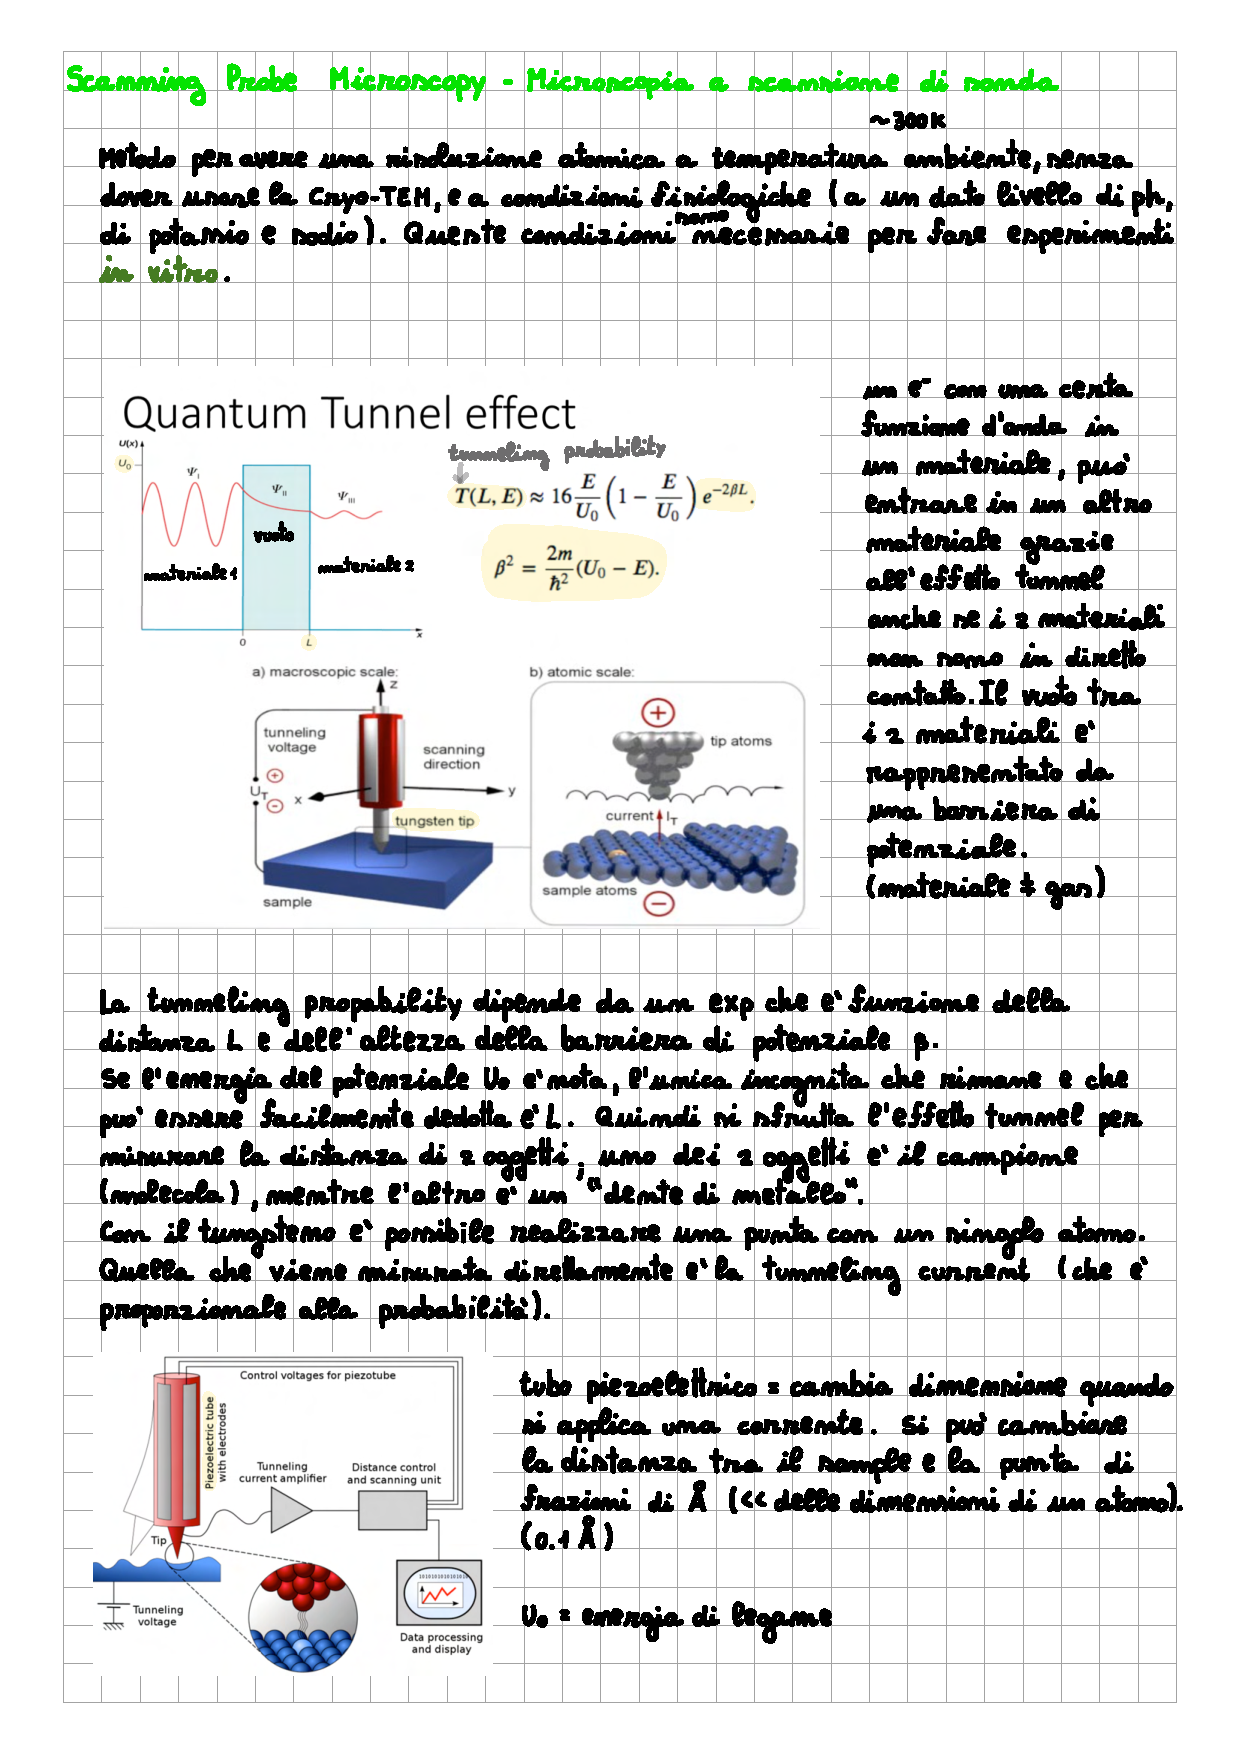
\includegraphics[width=\textwidth]{pics/02.png}
    \end{minipage}
    \caption{Andamento della magnetizzazione in funzione di $h$ e della temperature.}
    \label{fig:03-04}
\end{figure}


\noindent Il comportamento di $f(h)$ cambia a seconda della temperatura:
\begin{itemize}
    \item Per $T > T_c$, $f(h)$ è una funzione analitica e il suo sviluppo in serie di Taylor attorno a $h=0$ è:
    \begin{equation}
    f(h) = f(0) + c h^2 + O(h^4)
    \end{equation}
    \item Per $T < T_c$, la funzione presenta una singolarità (una cuspide) in $h=0$. Il suo sviluppo è:
    \begin{equation}
    f(h) = f(0) - m_s|h| + O(h^2)
    \end{equation}
    dove $m_s$ è la magnetizzazione spontanea. La derivata prima in $h=0$ è discontinua.
\end{itemize}

\subsection{Transizioni di Fase e Criterio di Ehrenfest}

Una transizione di fase si ha quando in corrispondenza di un valore preciso di un parametro del sistema, questo cambia drasticamente le sue proprietà (es. ghiaccio $\to$ acqua).

Il \textbf{Criterio di Ehrenfest} definisce l'ordine di una transizione di fase. Una transizione di fase è di ordine $k$ se l'energia libera $f$ è differenziabile $k-1$ volte, ma non $k$ volte.

\begin{itemize}
    \item Transizione di fase del primo ordine ($k=1$): L'energia libera $f$ è continua, ma la sua derivata prima (ad esempio, il volume o la magnetizzazione) è discontinua. Un esempio è la transizione acqua-ghiaccio.
    \item Transizione di fase del secondo ordine ($k=2$): La prima derivata dell'energia libera è continua, ma la seconda derivata è discontinua o singolare.
\end{itemize}


Nel modello di Ising, a $T=T_{c}$ si ha una \textbf{transizione di fase del secondo ordine in $T$}. In questo caso, la magnetizzazione $m_{Ising}$ (derivata prima di $f$ rispetto a $h$) non subisce un salto.

Al di sotto di $T_{c}$ ($T < T_{c}$), si ha una \textbf{transizione di fase del primo ordine in $h$} (cambiando il campo magnetico). Questo perché l'energia libera $f$ (o la sua derivata rispetto a $h$, che è $m$) salta quando si passa da $h=0^{-}$ a $h=0^{+}$.

\subsection{Lunghezza di Correlazione e Universalità}

Per $T > T_{c}$, all'aumentare della temperatura, la \textbf{lunghezza di correlazione} $\xi$ (che governa il decadimento delle funzioni di correlazione come $\langle \sigma_{i} \sigma_{j} \rangle \sim e^{-|i-j|/\xi}$ ) è molto piccola.

Quando la temperatura diminuisce e si avvicina a $T_{c}$, la lunghezza di correlazione $\xi$ aumenta, e a $T=T_{c}$, $\xi$ diventa infinita. In questo punto, la funzione di correlazione non decade più esponenzialmente, ma con una legge di potenza. L'esponenziale è il segno di una fisica locale.

Quando $\xi$ è infinita, una perturbazione locale può influenzare tutto il sistema (correlazione a raggio infinito).
L'infinita lunghezza di correlazione a $T_{c}$ implica che la fisica è dettata da grandi regioni dello spazio. Di conseguenza, i dettagli della struttura reticolare (lattice) diventano irrilevanti. Questo porta al concetto di \textbf{universalità}: sistemi molto diversi possono avere lo stesso comportamento critico.

\subsection{Teorema di Lee-Yang e Singolarità}

Per ottenere una singolarità nell'energia libera $f$ (che segnala una transizione di fase), si deve considerare il limite di volume infinito, $V \to \infty$.

Secondo il \textbf{Teorema di Lee-Yang}, una singolarità in $f(\beta)$ può svilupparsi solo se la funzione di partizione $\mathcal{Z}(\beta)$ ha uno zero nel piano complesso di $\beta$ o $h$.
\begin{equation}
f(\beta) = -\frac{1}{\beta V} \log(\mathcal{Z}(\beta)) \quad \to \quad \text{singolarità per } \mathcal{Z}=0
\end{equation}
La funzione di partizione $\mathcal{Z}$ è una funzione analitica  nel piano complesso di $\beta$ o $h$.

Per valori reali di $\beta$ (o temperatura $T$), per il modello di Ising a volume finito, $\mathcal{Z}$ non ha zeri. Infatti, $\mathcal{Z}$ è una somma di termini positivi $e^{-\beta E}$.

La singolarità si verifica quando gli zeri della funzione di partizione nel piano complesso (di $\beta$ o $h$) si avvicinano all'asse reale nel limite $V \to \infty$. Se la distanza dello zero più vicino all'asse reale non cambia con l'aumento di $V$, non si avrà una singolarità al limite $V \to \infty$. Se invece lo zero si avvicina all'asse reale (di $\beta$ o $h$) quando $V \to \infty$, allora al limite si sviluppa una singolarità nell'energia libera $f$.

Una singolarità in $f$ non significa necessariamente che $f$ è discontinua o che ha una divergenza, ma che non tutte le sue derivate sono definite o regolari. Una singolarità nella prima derivata di $f$ (che è una variabile di stato, come $m$) significa un impatto fisico.


\subsection{Ruolo delle condizioni al contorno}

A volume finito, per specificare il sistema, è necessario dare le condizioni al contorno.
\begin{itemize}
    \item B.C. positive ($+$ B.C.): tutti gli spin al contorno fissati a $+1$. 
    
    Per $T < T_{c}$, selezionano $m = m_{s}$.
    \item B.C. negative ($-$ B.C.): tutti gli spin al contorno fissati a $-1$. 
    
    Per $T < T_{c}$, selezionano $m = -m_{s}$.
    \item B.C. periodiche (Periodic B.C.): $m=0$. Queste condizioni minimizzano la differenza tra il sistema a volume finito e quello a volume infinito.
\end{itemize}

Quando c'è una transizione di fase del primo ordine, ci sono due o più stati stabili (ad esempio, $+m_{s}$ e $-m_{s}$ per il modello di Ising con $T < T_{c}$ e $h=0$). Le condizioni al contorno possono selezionare quale stato stabile viene raggiunto.

Una condizione al contorno è equivalente a un campo magnetico infinitesimale ($h$ infinitesimale) che rompe la simmetria. Infatti, anche se l'energia della superficie è infinitesima rispetto al volume, le B.C. positive selezionano lo stato positivo se $T < T_{c}$.

Nel limite $V \to \infty$, una volta che il sistema è nello stato $+m_{s}$, non c'è modo di passare allo stato $-m_{s}$, perché il costo energetico per creare un'interfaccia (un dominio) è infinito, e quindi il tempo di transizione è infinito.





